\documentclass[aps,prl,reprint,amsmath,amssymb]{revtex4-2}
\usepackage{tikz}
\usepackage{microtype}
\usepackage{placeins}
\usepackage{xurl}
\usetikzlibrary{arrows.meta,calc}
\hyphenpenalty=750
\tolerance=1200
\emergencystretch=1.5em

\begin{document}

\title{Continuation Geometry Resolves Apparent Family Splitting in Unequal-Mass Three-Body Orbits}

\author{Yossi Eliaz}
\affiliation{Incredibuild, Tel Aviv, Israel}
\affiliation{Department of Computer Science, Holon Institute of Technology, Holon, Israel}

\author{Ori Chemo}
\affiliation{Incredibuild, Tel Aviv, Israel}

\begin{abstract}
Periodic-orbit families are often represented through low-dimensional invariant
coordinates, whose projected branch structure need not preserve the connectivity
of the underlying solution manifold. We use numerical continuation to examine
the $135{,}445$ unequal-mass planar three-body periodic orbits reported by Li,
Li, and Liao, whose corrected scale-invariant period--angular-momentum
representation was subsequently interpreted as two independent sets. The two
projected branches belong to a single continuation-connected component, while
the invariant projection develops a singular locus associated with their
apparent separation. High-precision Floquet calculations identify a $(+1)$
transition at one representative stability boundary and an opposite-Krein
Hamiltonian--Hopf transition at another. The results show how projection
geometry can obscure periodic-orbit connectivity while the reduced symplectic
spectrum resolves the mechanisms governing stability changes.
\end{abstract}

\maketitle

Periodic orbits organize the dynamics of Hamiltonian systems.
As parameters vary, periodic solutions trace continuation manifolds whose
geometry and stability changes encode the surrounding dynamics.
Such families are commonly displayed through a small number of scalar
observables, including periods, actions, conserved quantities, or
scale-invariant combinations~\cite{chenciner2000figureeight,galan2002figureeight,li2025review}.
These diagrams are projections of the full solution set, so visible branch
structure can differ from continuation connectivity.
Distinguishing projected branches from connected components therefore requires
continuation in the underlying orbit space.

Li, Li, and Liao constructed $135{,}445$ unequal-mass non-hierarchical planar
periodic orbits on a mass grid with $m_3=1$, including $13{,}315$ samples
reported as linearly stable~\cite{li2021stable}.
They described the collection as one family.
Stan{\v c}evi{\'c}, Vasiljevi{\'c}, and Dmitra{\v s}inovi{\'c} identified two
distinct projected branches in the corrected scale-invariant
period--angular-momentum coordinates and interpreted them as independent
sets~\cite{stancevic2023moth}.
This raises a dynamical question: do those projected branches belong to
distinct continuation components of the periodic-orbit solution set?
All catalog members carry the same reported topological word; component
identity in this work is determined by continuation of periodic solutions.

We address this question by continuing periodic solutions directly through
mass and orbit space.
We then compute the reduced physical Floquet spectrum and represent its
stability boundaries through two symplectic trace
invariants~\cite{yakubovich1975,howard1987linear,frauenfelder2023symplectic}.
We study planar periodic orbits in the sampled Li--Li--Liao (LLL) continuation
with $m_3=1$; stability refers throughout to the nontrivial planar Floquet
spectrum of the reduced return map.
We use \emph{continuation component} for a connected set of periodic solutions
joined by the continuation procedure described below; when the historical term
\emph{family} is used, it refers to such a component unless explicitly
attributed to prior work.

The sampled solutions form one continuation-connected component, and a
continuation path joins the two branches visible in the scale-invariant
diagram.
The invariant projection contains a singular locus associated with their
apparent separation.
Along the same component, the physical Floquet spectrum exhibits a $(+1)$
transition and an opposite-Krein Hamiltonian--Hopf transition.
Three additional points satisfy the simultaneous $(+1)$ and $(-1)$ critical
conditions.
Together these results separate continuation connectivity from projected
branch structure and identify the distinct symplectic mechanisms underlying
representative stability changes.

% Figure 1. Schematic invariant projection and documented mass-space connection.
\begin{figure*}[t]
\centering
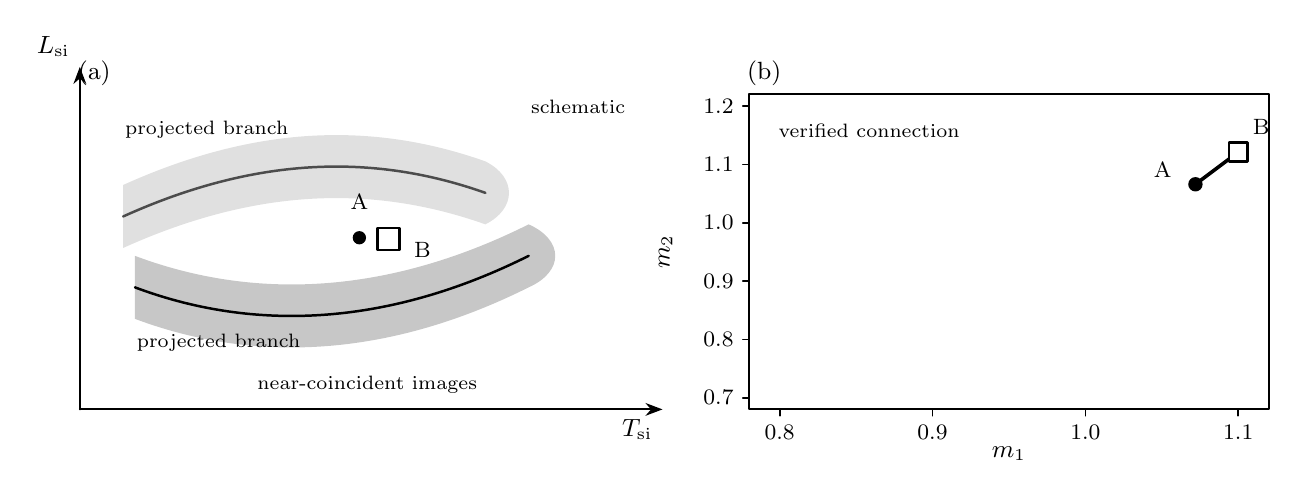
\begin{tikzpicture}[x=1cm,y=1cm,line cap=round,line join=round,
  >=Stealth,every node/.style={font=\footnotesize}]
  \begin{scope}
    \node[font=\small,anchor=north west] at (-0.15,4.55) {(a)};
    \draw[line width=0.7pt,->] (0,0) -- (7.4,0)
      node[below left,font=\small] {$T_{\rm si}$};
    \draw[line width=0.7pt,->] (0,0) -- (0,4.35)
      node[above left,font=\small] {$L_{\rm si}$};
    \fill[black!12]
      (0.55,2.85) .. controls (2.1,3.55) and (3.6,3.70) .. (5.15,3.15)
      .. controls (5.55,2.95) and (5.55,2.55) .. (5.15,2.35)
      .. controls (3.6,2.90) and (2.1,2.75) .. (0.55,2.05) -- cycle;
    \fill[black!22]
      (0.70,1.15) .. controls (2.3,0.55) and (4.0,0.70) .. (5.70,1.55)
      .. controls (6.15,1.75) and (6.15,2.15) .. (5.70,2.35)
      .. controls (4.0,1.50) and (2.3,1.35) .. (0.70,1.95) -- cycle;
    \draw[line width=0.9pt,black!70]
      (0.55,2.45) .. controls (2.1,3.15) and (3.6,3.30) .. (5.15,2.75);
    \draw[line width=0.9pt,black]
      (0.70,1.55) .. controls (2.3,0.95) and (4.0,1.10) .. (5.70,1.95);
    \fill[black] (3.55,2.18) circle (2.4pt);
    \draw[line width=0.8pt,black,fill=white]
      (3.78,2.02) rectangle ++(0.28,0.28);
    \node[anchor=south] at (3.55,2.42) {A};
    \node[anchor=west] at (4.12,2.02) {B};
    \node[align=center,font=\scriptsize,anchor=north] at (3.65,0.55)
      {near-coincident images};
    \node[font=\scriptsize,anchor=west] at (0.45,3.55) {projected branch};
    \node[font=\scriptsize,anchor=west] at (0.60,0.85) {projected branch};
    \node[font=\scriptsize,anchor=north east] at (7.05,4.05) {schematic};
  \end{scope}

  \begin{scope}[shift={(8.5,0)}]
    \node[font=\small,anchor=north west] at (-0.15,4.55) {(b)};
    \draw[line width=0.7pt] (0,0) rectangle (6.6,4.0);
    \foreach \m/\lab in {0.388/0.8,2.329/0.9,4.271/1.0,6.212/1.1}
      \draw[line width=0.6pt] (\m,-0.08) -- (\m,0)
        node[below=2pt] {$\lab$};
    \foreach \m/\lab in {0.148/0.7,0.889/0.8,1.630/0.9,2.370/1.0,3.111/1.1,3.852/1.2}
      \draw[line width=0.6pt] (-0.08,\m) -- (0,\m)
        node[left=2pt] {$\lab$};
    \node[below=10pt,font=\small] at (3.3,0) {$m_1$};
    \node[rotate=90,anchor=south,font=\small] at (-0.85,2.0) {$m_2$};
    \coordinate (A) at (5.668,2.859);
    \coordinate (B) at (6.212,3.267);
    \draw[line width=1.3pt,black] (A) -- (B);
    \fill[black] (A) circle (2.6pt);
    \draw[line width=0.9pt,black,fill=white]
      (B) ++(-0.12,-0.12) rectangle ++(0.24,0.24);
    \node[anchor=east] at ($(A)+(-0.18,0.18)$) {A};
    \node[anchor=south west] at ($(B)+(0.06,0.10)$) {B};
    \node[font=\scriptsize,align=left,anchor=north west] at (0.25,3.75)
      {verified connection};
  \end{scope}
\end{tikzpicture}
\caption{\label{fig:projection}Continuation connectivity and invariant projection.
(a)~Schematic of the two branches visible in the corrected scale-invariant
period--angular-momentum representation. The documented long-range pair A and
B has nearly coincident invariant images. (b)~The same pair in the
$(m_1,m_2)$ plane. The line denotes the verified bidirectional continuation
connection between the endpoints; its drawn shape is schematic. Their mass
distance is $0.062$. The projected branch separation therefore occurs within
one continuation-connected sampled solution set.}
\end{figure*}


\emph{Continuation geometry.}---We continue the periodic solutions in the mass
parameters $(m_1,m_2)$ at fixed $m_3=1$.
A periodic solution at one mass point supplies the predictor for a neighboring
point, followed by correction of the orbit and period to restore periodicity.
Repeating this procedure traces connected branches through the sampled orbit
set.

The mass-adjacency graph of the $135{,}445$ sampled solutions is connected.
It contains $270{,}087$ mass-adjacent links and admits a spanning tree with
$135{,}444$ edges.
We selected $26$ connections that maximize indicators of possible branch
separation: five macroscopic graph bottlenecks, the twenty largest chart
discontinuities along the spanning tree, and one long-range cross-branch
connection associated with nearly coincident invariant coordinates.
Bidirectional continuation succeeds across all $26$ selected connections.
The long-range cross-branch connection was also reproduced in a
translation-reduced strict-periodic formulation.

A path through the sampled continuation component connects representative
solutions on the two branches of the $(T_{\rm si},L_{\rm si})$ diagram
[Fig.~\ref{fig:projection}].
The visible branch separation therefore occurs inside one continuation-connected
sampled solution set.

The corrected scale-invariant period and angular momentum define the invariant
projection
\begin{equation}
\Psi(m_1,m_2)=(T_{\rm si},L_{\rm si}),
\end{equation}
where $T_{\rm si}=T\lvert E\rvert^{3/2}M^{-5/2}$ and
$L_{\rm si}=L\lvert E\rvert^{1/2}M^{-13/6}$ are the mass-corrected period and
angular momentum, with $M=m_1+m_2+m_3$.
Finite-difference estimates of $D\Psi$ identify adjacent mass cells across
which $\det D\Psi$ changes sign.
These sign changes assemble into a singular locus in the sampled mass plane.
The audit also finds far-separated mass points whose scale-invariant
coordinates are nearly coincident.
The discrete audit contains $590$ determinant-sign-change edges and $86$
long-range near coincidences under the stated thresholds.
Together these observations identify projection geometry as the origin of the
apparent separation between the two visible branches.

\emph{Floquet stability.}---After removal of the neutral symmetry directions,
each periodic orbit has four nontrivial Floquet multipliers forming two
reciprocal pairs.
The corresponding $4\times 4$ symplectic return map can be represented by two
trace invariants $(\alpha,\beta)$.
With $t=\lambda+\lambda^{-1}$, the spectral polynomial is
\begin{equation}
P(t)=t^2-(\alpha-4)t+\beta-4\alpha+8,
\end{equation}
and the three spectral boundaries are
\begin{align}
G_+&=\beta-6\alpha+20,\\
G_-&=\beta-2\alpha+4,\\
\Delta&=\alpha^2+8\alpha-16-4\beta.
\end{align}
The conditions $G_+=0$ and $G_-=0$ correspond to multipliers at $+1$ and $-1$,
respectively, while $\Delta=0$ marks a collision of the two reciprocal mode
traces.
The critical curves in mass space are preimages of these spectral boundaries
under
\begin{equation}
\Phi(m_1,m_2)=(\alpha,\beta).
\end{equation}
We use this standard symplectic trace representation to distinguish the
mechanisms of the observed stability
transitions~\cite{yakubovich1975,howard1987linear}.

Symplecticity pairs each nontrivial multiplier $\lambda$ with $\lambda^{-1}$.
For an elliptic multiplier on the unit circle, the Krein signature gives the
sign of the associated symplectic quadratic form.

% Figure 2. Distinct Floquet mechanisms from committed 60-digit flanks.
\begin{figure*}[t]
\centering
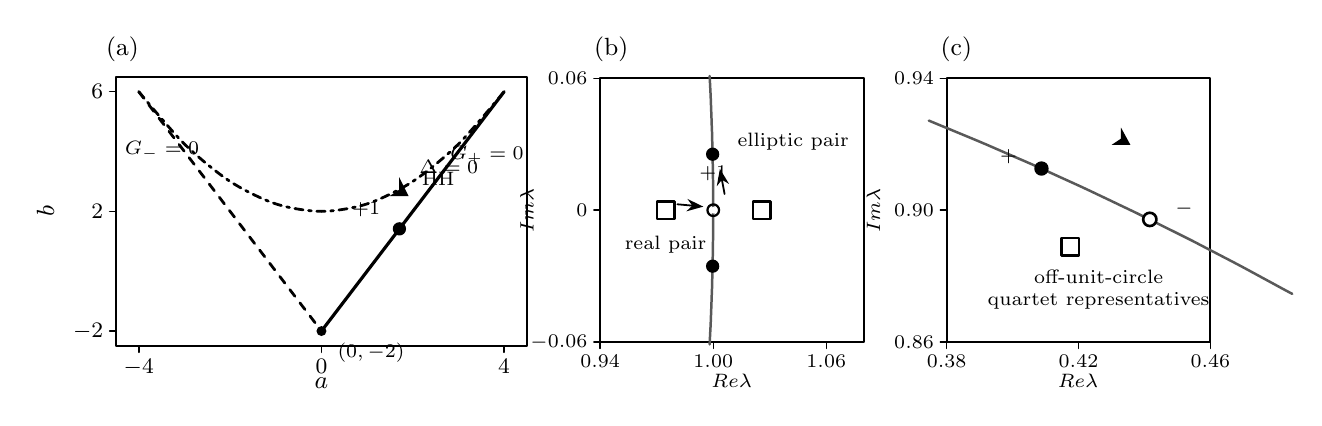
\begin{tikzpicture}[x=1cm,y=1cm,line cap=round,line join=round,
  >=Stealth,every node/.style={font=\footnotesize}]
  % ============================================================
  % (a) physical Sp(4) trace plane
  % a in [-4.5,4.5], b in [-2.5,6.5]
  % x = 0.58(a+4.5), y = 0.38(b+2.5)
  % ============================================================
  \begin{scope}
    \node[font=\small,anchor=north west] at (-0.25,4.05) {(a)};
    \draw[line width=0.75pt] (0,0) rectangle (5.22,3.42);
    \foreach \x/\lab in {0.29/-4,2.61/0,4.93/4}
      \draw[line width=0.55pt] (\x,-0.08) -- (\x,0)
        node[below=1pt] {$\lab$};
    \foreach \y/\lab in {0.19/-2,1.71/2,3.23/6}
      \draw[line width=0.55pt] (-0.08,\y) -- (0,\y)
        node[left=1pt] {$\lab$};
    \node[below=8pt,font=\small] at (2.61,0) {$a$};
    \node[rotate=90,anchor=south,font=\small] at (-0.66,1.71) {$b$};

    % Delta=0: b=a^2/4+2
    \draw[line width=1.0pt,dash dot]
      plot[smooth] coordinates {
        (0.29,3.23) (0.87,2.565) (1.45,2.09) (2.03,1.805)
        (2.61,1.71) (3.19,1.805) (3.77,2.09) (4.35,2.565)
        (4.93,3.23)
      };
    % G-=0: b=-2a-2 from (-4,6) to (0,-2)
    \draw[line width=1.0pt,dashed] (0.29,3.23) -- (2.61,0.19);
    % G+=0: b=2a-2 from (0,-2) to (4,6)
    \draw[line width=1.15pt] (2.61,0.19) -- (4.93,3.23);
    \node[font=\scriptsize,anchor=west] at (4.12,2.42) {$G_+=0$};
    \node[font=\scriptsize,anchor=east] at (1.18,2.48) {$G_-=0$};
    \node[font=\scriptsize,anchor=west] at (3.73,2.28) {$\Delta=0$};

    % mixed vertex (a,b)=(0,-2)
    \fill[black] (2.61,0.19) circle (1.8pt);
    \node[font=\scriptsize,anchor=north west] at (2.69,0.16) {$(0,-2)$};

    % +1 event: a=1.7065, b=1.4145 -> x=3.5998, y=1.4875
    \fill[black] (3.600,1.488) circle (2.4pt);
    \node[font=\scriptsize,anchor=east] at (3.48,1.73) {$+1$};

    % HH event: a=1.7007, b=2.7242 -> x=3.5964, y=1.9852
    \fill[black] (3.596,1.985) -- ++(0.00,0.16)
      -- ++(0.12,-0.24) -- ++(-0.24,0) -- cycle;
    \node[font=\scriptsize,anchor=west] at (3.76,2.12) {HH};
  \end{scope}

  % ============================================================
  % (b) zoom near +1
  % Re lambda in [0.94,1.08], Im lambda in [-0.06,0.06]
  % ============================================================
  \begin{scope}[shift={(6.15,0.05)}]
    \node[font=\small,anchor=north west] at (-0.20,4.00) {(b)};
    \draw[line width=0.75pt] (0,0) rectangle (3.35,3.35);
    \foreach \x/\lab in {0.000/0.94,1.436/1.00,2.871/1.06}
      \draw[line width=0.55pt] (\x,-0.08) -- (\x,0)
        node[below=1pt,font=\scriptsize] {$\lab$};
    \foreach \y/\lab in {0.000/-0.06,1.675/0,3.350/0.06}
      \draw[line width=0.55pt] (-0.08,\y) -- (0,\y)
        node[left=1pt,font=\scriptsize] {$\lab$};
    \node[below=8pt,font=\scriptsize] at (1.67,0)
      {$\operatorname{Re}\lambda$};
    \node[rotate=90,anchor=south,font=\scriptsize] at (-0.72,1.67)
      {$\operatorname{Im}\lambda$};
    \draw[line width=0.9pt,black!65]
      plot[domain=-3.5:3.5,samples=60]
        ({(cos(\x)-0.94)/0.14*3.35},{(sin(\x)+0.06)/0.12*3.35});
    \draw[line width=0.8pt] (1.436,1.675) circle (2.1pt);
    \fill[white] (1.436,1.675) circle (1.2pt);
    \node[font=\scriptsize,anchor=south] at (1.436,1.92) {$+1$};

    % unstable real reciprocal pair
    \draw[line width=0.9pt,fill=white]
      (0.833,1.675) ++(-0.11,-0.11) rectangle ++(0.22,0.22);
    \draw[line width=0.9pt,fill=white]
      (2.053,1.675) ++(-0.11,-0.11) rectangle ++(0.22,0.22);
    \node[font=\scriptsize,anchor=north] at (0.83,1.47) {real pair};

    % stable unit-circle pair
    \fill[black] (1.428,2.386) circle (2.4pt);
    \fill[black] (1.428,0.964) circle (2.4pt);
    \node[font=\scriptsize,anchor=west] at (1.62,2.55) {elliptic pair};

    \draw[->,line width=0.65pt] (0.98,1.75) -- (1.31,1.72);
    \draw[->,line width=0.65pt] (1.58,1.88) -- (1.52,2.20);
  \end{scope}

  % ============================================================
  % (c) zoom of opposite-Krein collision, upper half-plane
  % Re in [0.38,0.46], Im in [0.86,0.94]
  % ============================================================
  \begin{scope}[shift={(10.55,0.05)}]
    \node[font=\small,anchor=north west] at (-0.20,4.00) {(c)};
    \draw[line width=0.75pt] (0,0) rectangle (3.35,3.35);
    \foreach \x/\lab in {0.000/0.38,1.675/0.42,3.350/0.46}
      \draw[line width=0.55pt] (\x,-0.08) -- (\x,0)
        node[below=1pt,font=\scriptsize] {$\lab$};
    \foreach \y/\lab in {0.000/0.86,1.675/0.90,3.350/0.94}
      \draw[line width=0.55pt] (-0.08,\y) -- (0,\y)
        node[left=1pt,font=\scriptsize] {$\lab$};
    \node[below=8pt,font=\scriptsize] at (1.67,0)
      {$\operatorname{Re}\lambda$};
    \node[rotate=90,anchor=south,font=\scriptsize] at (-0.72,1.67)
      {$\operatorname{Im}\lambda$};
    \draw[line width=0.9pt,black!65]
      plot[domain=61:68,samples=40]
        ({(cos(\x)-0.38)/0.08*3.35},{(sin(\x)-0.86)/0.08*3.35});

    % stable modes and Krein signs
    \fill[black] (1.204,2.204) circle (2.6pt);
    \node[font=\scriptsize,anchor=east] at (1.02,2.35) {$+$};
    \draw[line width=0.95pt,fill=white] (2.580,1.558) circle (2.4pt);
    \node[font=\scriptsize,anchor=west] at (2.78,1.70) {$-$};

    % upper-half representatives of unstable quartet
    \draw[line width=0.9pt,fill=white]
      (1.568,1.209) ++(-0.11,-0.11) rectangle ++(0.22,0.22);
    \fill[black] (2.214,2.584) -- ++(0.00,0.14)
      -- ++(0.12,-0.22) -- ++(-0.24,0) -- cycle;
    \node[font=\scriptsize,align=center] at (1.93,0.67)
      {off-unit-circle\\quartet representatives};
  \end{scope}
\end{tikzpicture}
\caption{\label{fig:floquet}Distinct Floquet mechanisms on the continuation
component. (a)~Stability geometry in the physical $\operatorname{Sp}(4)$ trace
plane. The boundaries $G_+=0$ (solid), $G_-=0$ (dashed), and $\Delta=0$
(dot-dashed) correspond to $+1$, $-1$, and mode-collision conditions. The
filled circle marks the lower $+1$ transition and the filled triangle the upper
Hamiltonian--Hopf transition; the mixed vertex is $(a,b)=(0,-2)$.
(b)~Near the lower boundary, a real reciprocal pair (open squares) reaches
$+1$ and becomes an elliptic unit-circle pair (filled circles).
(c)~On the stable flank of the upper boundary, two unit-circle modes have
opposite Krein signatures (filled $+$ and open $-$). Beyond their collision,
the upper-half representatives lie on opposite sides of the unit circle; their
conjugates complete a reciprocal complex quartet.}
\end{figure*}


\emph{Stability transitions.}---Along $m_1=0.8023446$, the lower representative
stability boundary occurs near $m_2=0.75401872$.
On the unstable side, the relevant Floquet modes form a real reciprocal pair.
Approaching the boundary, the pair reaches $+1$; beyond the boundary it lies on
the unit circle [Fig.~\ref{fig:floquet}(b)].
An independent $60$-digit implementation reproduces the transition within an
$m_2$ bracket of width $1.6\times10^{-9}$.

Along $m_1=0.8022890$, two elliptic Floquet modes approach one another on the
unit circle at the upper representative stability boundary.
Their Krein signatures have opposite signs on the stable side.
At the boundary the modes collide, and beyond it the spectrum forms a
reciprocal complex quartet off the unit circle [Fig.~\ref{fig:floquet}(c)].
The transition is therefore an opposite-Krein Hamiltonian--Hopf instability.
The independent $60$-digit calculation reproduces the critical location within
an $m_2$ bracket of width $6.3\times10^{-9}$.

The $+1$ and $-1$ spectral boundaries meet at $(\alpha,\beta)=(4,4)$.
Solving the simultaneous conditions $G_+=G_-=0$ yields three mixed spectral
intersections in the sampled mass domain.
The intersections occur near $(m_1,m_2)=(0.929239,0.885366)$,
$(0.996768,0.956019)$, and $(1.049553,1.129476)$.
All three were recomputed at $60$-digit precision with small shooting and
spectral residuals.

Direct continuation connects the two branches of the corrected scale-invariant
period--angular-momentum representation within one sampled component of the LLL
periodic-orbit manifold.
A singular locus of the invariant projection provides the geometric origin of
their apparent separation.
The physical Floquet spectrum distinguishes a $+1$ transition from an
opposite-Krein Hamiltonian--Hopf transition along the same continuation
component.
Three additional mass points map to the mixed $+1/-1$ spectral vertex.
The example shows that projected branch structure and continuation
connectivity encode different information about a periodic-orbit family.
Continuation resolves the organization of the periodic solutions, while the
symplectic spectrum identifies the mechanisms through which their stability
changes.
The same distinction is relevant whenever a multidimensional periodic-orbit
family is classified through a small number of projected invariants.

\FloatBarrier
\section*{Acknowledgments}
xAI Grok (version 4.6) was used to assist with manuscript organization and
revision of scientific exposition.
AI coding agents operating in islo.dev sandboxes assisted, under the authors'
direction, with development of the analysis software that generated the
committed numerical records.
All calculations reported here were executed by the deterministic numerical
programs described in the End Matter; the authors reviewed the AI-assisted
text and software against those records, the source data, and the cited
literature, and take responsibility for the final scientific statements and
conclusions.

\section*{Data Availability}

The numerical data and software supporting the analyses reported here are
publicly available in Ref.~\cite{eliaz2026archive}.
The upstream orbit catalog is available from Ref.~\cite{li2021stable} and is
not redistributed with the archive.

\clearpage
\appendix
\section*{End Matter}

\section{\label{app:continuation}Numerical continuation}

Planar Newtonian motion with $G=1$ is
\begin{equation}
\ddot{\mathbf{r}}_i=\sum_{j\neq i}
m_j\frac{\mathbf{r}_j-\mathbf{r}_i}{\lvert\mathbf{r}_j-\mathbf{r}_i\rvert^3}.
\end{equation}
The LLL catalog is continued at fixed~$m_3=1$ over the published mass window
$m_1\in[0.8,1.1]$, $m_2\in[0.7,1.2]$.
Published samples occupy the collinear shooting chart
\begin{equation}
\begin{aligned}
\mathbf r_1&=(x_1,0),\quad \mathbf r_2=(1,0),\quad \mathbf r_3=(0,0),\\
\mathbf v_1&=(0,v_1),\quad \mathbf v_2=(0,v_2),
\end{aligned}
\end{equation}
with $\mathbf v_3$ fixed by vanishing total momentum.
The shooting unknowns at fixed masses are $(x_1,v_1,v_2,T)$.
A neighboring catalog point supplies the predictor; a Newton corrector restores
periodicity in the eight-dimensional center-of-mass-reduced coordinates.
The closure residual is the reduced return defect after one period.
A connection is recorded when bidirectional continuation between two mass
points converges and the terminal shooting charts match.

The long-range cross-branch connection joins the catalog samples at
$(m_1,m_2)=(1.072,1.066)$ and $(1.100,1.121)$, a Euclidean mass distance of
$0.0617$.
Eighty continuation steps in each direction close with shooting residual below
$2.3\times10^{-10}$ and terminal chart mismatch below $6\times10^{-13}$.
The same pair was recomputed in a translation-reduced strict-periodic
formulation outside the collinear-velocity ansatz.

\section{\label{app:floquet}Physical Floquet calculation}

After center-of-mass reduction the variational equation is integrated in
canonical Jacobi coordinates
$(\boldsymbol\rho,\boldsymbol\lambda,\mathbf p_{\rho},\mathbf p_{\lambda})$,
with
\begin{equation}
\boldsymbol\rho=\mathbf r_2-\mathbf r_1,\qquad
\boldsymbol\lambda=\mathbf r_3-\frac{m_1\mathbf r_1+m_2\mathbf r_2}{m_1+m_2}.
\end{equation}
The resulting eight-dimensional monodromy is symplectic.
The two-dimensional subspace
$E=\mathrm{span}\{X_H,X_L\}$ generated by the Hamiltonian and angular-momentum
vector fields is removed by passing to the physical quotient $E^{\omega}/E$.
The reduced return map is a $4\times 4$ symplectic matrix $M$ whose spectrum
comprises the four nontrivial Floquet multipliers.
The trace invariants are
\begin{equation}
\alpha=\mathrm{tr}\,M,\qquad
\beta=\bigl((\mathrm{tr}\,M)^2-\mathrm{tr}(M^2)\bigr)/2,
\end{equation}
and they determine $P(t)$ as in the main text.
On a unit-circle eigenmode the Krein signature is the sign of the associated
symplectic quadratic form.
Closure and symplectic defects quoted below are the reduced periodic-return
norm and the departure of $M$ from $\mathrm{Sp}(4)$, respectively.

\section{\label{app:precision}High-precision verification}

The two representative transitions were recomputed in an independent
implementation using $60$-digit arithmetic and a ninth-order Verner integrator
in the Jacobi chart, followed by the physical quotient.
Each transition is enclosed by a sign-changing numerical bracket of the event
function in $m_2$.
On the lower $(+1)$ flanks the reduced closure is of order $10^{-21}$ and the
physical symplectic defect is of order $10^{-19}$.
On the Hamiltonian--Hopf flanks the corresponding figures are $10^{-22}$ and
$10^{-20}$.
The three mixed intersections were obtained by a simultaneous Newton solve of
$G_+=G_-=0$ in the same $60$-digit implementation; relative event residuals lie
between $10^{-14}$ and $10^{-13}$.

The connectivity statement concerns the sampled LLL continuation under the
chart and corrector above.
The numerical Jacobian estimate of $\Psi$ is a centered finite-difference
audit of the published mass grid.

\bibliography{references}

\end{document}
